\documentclass{article}%
\usepackage{fancyhdr}
\usepackage[a4paper, top=2.5cm, bottom=2.5cm, left=2.2cm, right=2.2cm]%
{geometry}
\usepackage{amsmath}
\usepackage{changepage}
\usepackage{amssymb}
\usepackage{graphicx}%

\newenvironment{proof}[1][Proof]{\textbf{#1.} }{\ \rule{0.5em}{0.5em}}

\newcommand{\Q}{\mathbb{Q}}
\newcommand{\R}{\mathbb{R}}
\newcommand{\C}{\mathbb{C}}
\newcommand{\Z}{\mathbb{Z}}

\begin{document}

\title{Homework 4}
\author{Ted Xiao}
\date{\today}
\maketitle

\section{Continuous Policy Gradient}
\begin{figure}[h]
    \center
		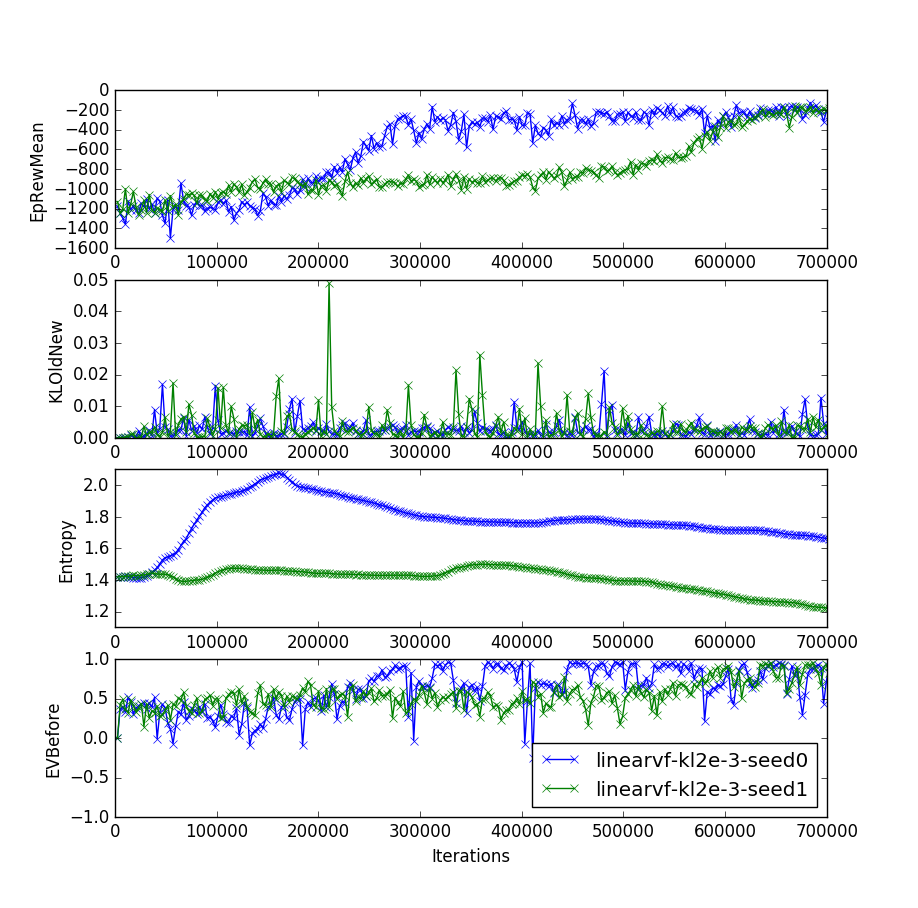
\includegraphics[width=0.9\textwidth]{linearvf_plot4.png}
    \caption{Continuous policy gradients applied to the Pendulum environment. Both seeds converge to rewards of at least $-300$. I used the default hyperparameters, but cut off the plot as soon as the results converged, which was at around $700000$ steps. The default hyperparameters used were: $\gamma = 0.97$, n\_iter=$300$,initial\_stepsize=1e-3, desired\_kl=2e-3, min\_timesteps\_per\_batch=$2500$. As seen above, the algorithm learned in around $650000$ to $700000$ steps.}
\end{figure}

            
\newpage
\section{Neural Network Value Function}

\begin{figure}[h]
    \center
		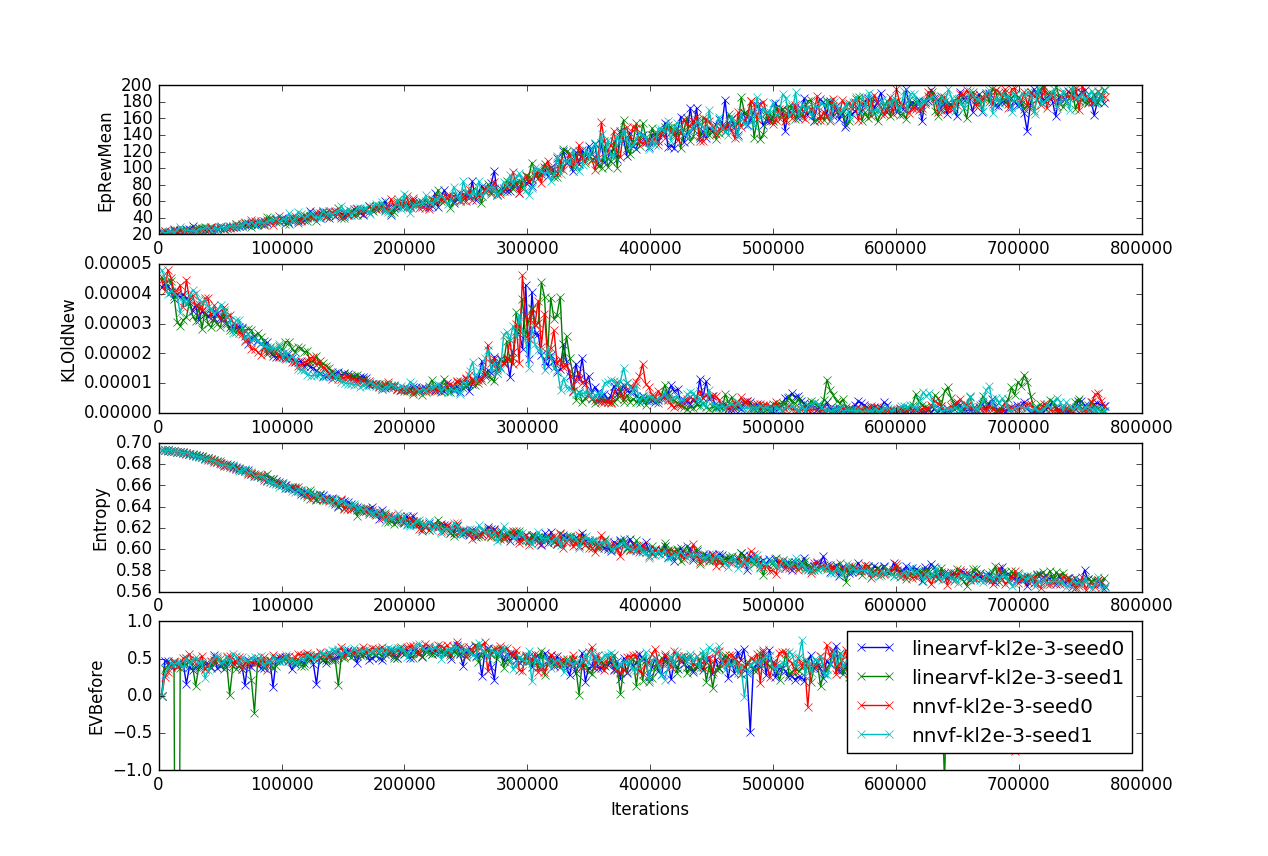
\includegraphics[width=0.9\textwidth]{nnvf_cartpole.png}
    \caption{The Neural Network Value function performs marginally better than the Linear Value Function on the cartpole task. The Neural Network Value function converges faster and has less variance overall. For the hyperparameters, the default training parameters were used: n\_epochs=10, stepsize=1e-3. The architecture was a simple two hidden layer feedforward neural network, with one hidden layer of 32 neurons and the second layer of 16 neurons.}
\end{figure}

\begin{figure}[h]
    \center
		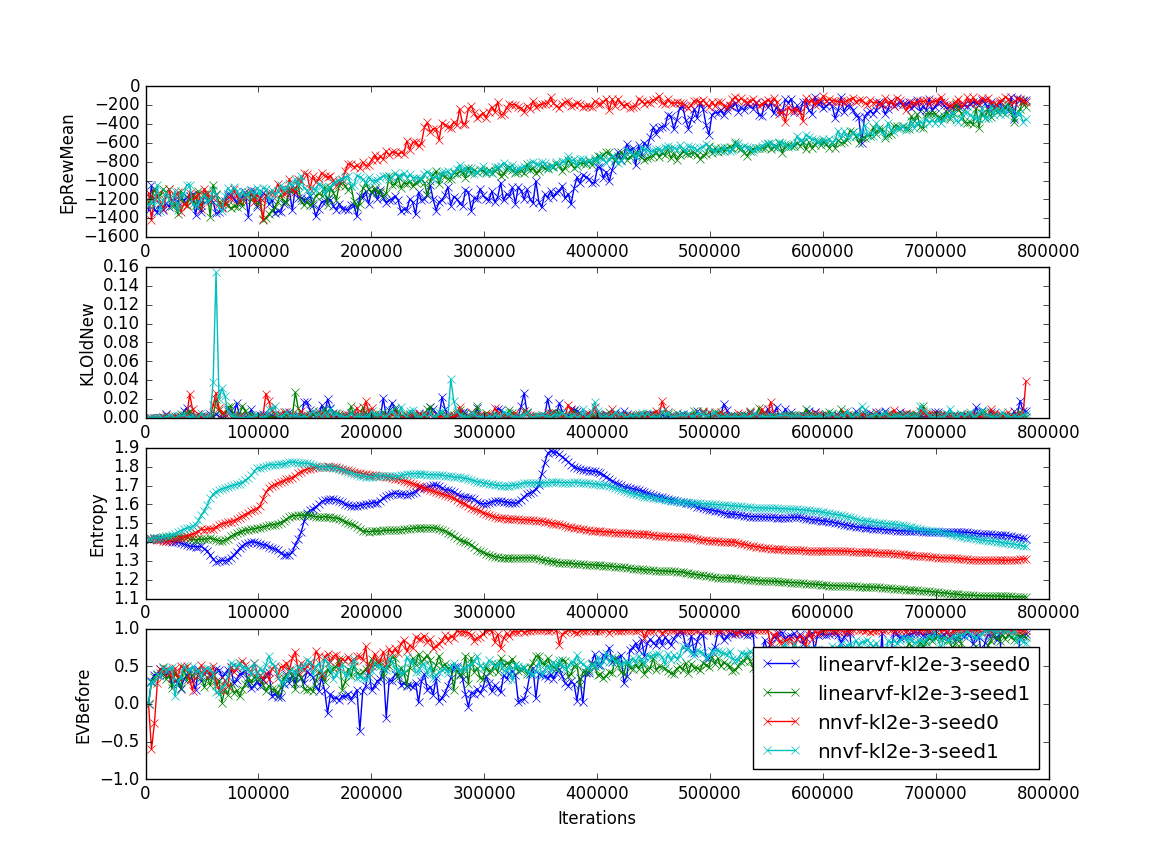
\includegraphics[width=0.9\textwidth]{nnvf_pendulum.png}
    \caption{The Neural Network Value function performs much better than the Linear Value Function on the pendulum task. The overall mean episode reward increases much faster than the linear value function. This may be because the task is harder to learn for a linear matrix model, so a neural network is better able to learn this more complex task. For the hyperparameters, the default training parameters were used: n\_epochs=10, stepsize=1e-3. The architecture was a simple two hidden layer feedforward neural network, with one hidden layer of 32 neurons and the second layer of 16 neurons.}
\end{figure}


\end{document}